
\vspace{-0.1cm}
\section{Problem Setting and Model Functions}
\label{sec:problem-setting}





\paragraph{Problem setting}
Let the input space $\gX$ be a discrete and countable set, and the output space $\gY$ be a discrete and finite set. We define the space of all possible datasets as $\gD = (\gX \times \gY)^*$, the set of all finite sequences of input-output pairs. For any dataset $D = ((x_1, y_1), \ldots, (x_n, y_n)) \in \gD$, we denote the corresponding sequence of inputs as $X = (x_1, \ldots, x_n)$ and outputs as $Y = (y_1, \ldots, y_n)$. Our analysis focuses on properties of encoding schemes that hold for any such pair of sequences $(X,Y)$.

\vspace{-0.1cm}

\paragraph{Model functions}

Neural networks modeling distributions over a discrete output space are typically characterized by a \emph{model function}, $f$, which defines a conditional distribution over a discrete space $\gY$ by mapping an input $x \in \gX$ to a vector of unnormalized logits, $f(x) \in \gL$. Motivated by the finite-precision arithmetic used in neural networks, we assume these logits are rational numbers (i.e. $\gL = \mathbb{Q}^{|\gY|}$) which enables a straightforward definition for the Kolmogorov complexity of a model function, $K(f)$.\footnote{See Appendix~\ref{sec:real-valued-distributions} for a discussion of the complexities involved with real-valued functions.}
We denote the set of all such computable model functions as $\gF$. The conditional distribution for a function $f \in \gF$ is given by applying the softmax function, $\sigma$, to its output logits:
\begin{align}
p(Y \mid X;f) = \prod_{x,y \in X,Y} p(y \mid x;f) &&
p(y \mid x;f) = \sigma(f(x))_y \label{eq:softmax}
\end{align}
In the following sections, we apply the MDL principle to this setting, where we want to identify \emph{codes} that select for a probabilistic model of this form that optimally compresses a set of labels $Y$ given corresponding inputs $X$, yielding a \emph{description length objective}.



\vspace{-0.1cm}
\section{Two-Part Codes} 
\label{sec:two-part-codes}
\vspace{-0.1cm}

One way to apply the MDL principle is with two-part codes. Consider the cost for a sender (e.g., Alice) to transmit labels $Y$ to a receiver (e.g., Bob), if both are given the inputs $X$. With a \emph{two-part code}, Alice first transmits a model hypothesis, and then transmits the labels encoded given this model hypothesis (Figure~\ref{fig:two_part_code}). Specifically, we consider two-part codes that are parameterized by a probabilistic model function (Section~\ref{sec:problem-setting}), which we refer to simply as \emph{two-part codes} in this paper.

\begin{defn}[two-part code] A \emph{two-part code} $M$ is specified by a triplet $\langle \gH_M, m_M, \alpha_M \rangle$ with:%
\begin{itemize}
    \item A hypothesis space $\gH_M$ which we assume is countable, e.g., the parameter space of a particular neural network assuming parameters with some finite-precision.
    \item A mapping $m_M : \gH_M \rightarrow \gF$ from hypotheses to model functions (Section~\ref{sec:problem-setting}), e.g., the mapping defined by a particular neural network architecture.\footnote{This can be a partial function, e.g. a Turing machine with unbounded resources may never halt for some inputs.}
    \item A prior $\alpha_M(h)$ defining a distribution over model hypotheses, $\gH_M$.\footnote{Formally we allow the prior to be any lower semicomputable semimeasure (see Appendix \ref{sec:app-background}).}
\end{itemize}
\label{def:two-part-code}\end{defn}


\begin{figure}[t!]
    \centering
    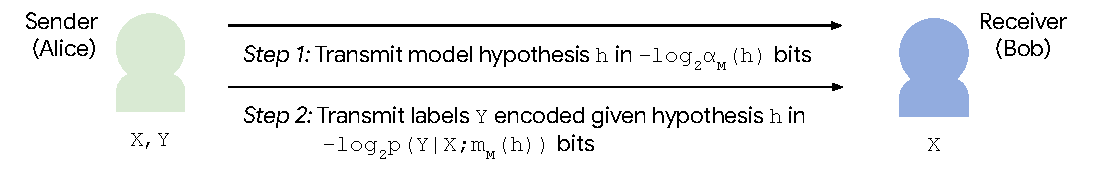
\includegraphics[width=0.85\columnwidth,keepaspectratio]{figures/two_part_code_pdf.pdf}
    \caption{\textbf{Two-part code.} One way to formalize the MDL principle is with a two-part code. %
    Assume Alice and Bob agree on a two-part code $M$ and each are given inputs $X$. Alice then finds the hypothesis (e.g., model parameters) that enables sending Bob the labels $Y$ in the fewest total bits, balancing the complexity of the model with how well it fits the data. One key challenge we address is that the minimum codelength is dependent on the potentially arbitrary choice of prior $\alpha_M(h)$. %
    }
    \label{fig:two_part_code}
\end{figure}


Given a two-part code $M$, the codelength for transmitting $Y$ given $X$ is defined as the sum of the codelength of the hypothesis and the codelength of the data given the hypothesis:
\begin{align}
    L_{M}^{\text{two-part}}(Y \mid X;h) &= -\log_2 \alpha(h) -\log_2 p(Y \mid X;m_M(h)).
    \label{eq:two-part-code}
\end{align}
The $-\log_2$ terms represent the ideal codelength for transmitting the model and data under the distributions specified by the prior and the selected hypothesis, respectively; the latter term is recognizable as the standard negative log-likelihood (NLL) objective. From a Bayesian perspective, 
minimizing \eqref{eq:two-part-code} can be interpreted as finding the MAP estimate.
The minimum achievable codelength for transmitting the labels with the two-part code $M$ is then denoted as:
\begin{equation}
    L_M^{\bigast,\text{two-part}}(Y \mid X) = \min_{h \in \gH_M}
    L_M^{\text{two-part}}(Y \mid X;h).
    \label{eq:two-part-min}
\end{equation}

\paragraph{Universal two-part codes}

Notably, there is a considerable degree of freedom in specifying a two-part code, e.g. for a particular neural network architecture specifying the hypothesis space and mapping function, we can choose any prior over the model weights. The prior determines the description length measure over the weights, which, in effect, determines the inductive bias of the codelength objective.
Building on the invariance theorem for Kolmogorov complexity, we will show that there exists an equivalence class of two-part codes that are \emph{universal} in the sense that a minimizer of any universal two-part code offers at least as much compression as any other two-part code, for any dataset, up to an additive constant that does not depend on the data. This guarantee holds regardless of the specific prior, as long as it constructs a universal code, and is captured in the following theorem and its corollary.

\begin{defn}[universal two-part code]
Let $M^1$ be a two-part code. $M^1$ is a \emph{universal two-part code} if and only if, for any other two-part code, $M^2$, the following holds for any dataset $X,Y$:
\begin{equation}
L^{\bigast,\text{two-part}}_{M^1}(Y \mid X) \leqc L^{\bigast,\text{two-part}}_{M^2}(Y \mid X).
\end{equation}
\end{defn}

\begin{prop}
There exists a universal two-part code.
\label{thm:universal-two-part-existence}
\end{prop}

\begin{cor}\label{thm:universal-two-part-min} The minimum of any universal two-part code $M$ is equal to the following bound, denoted $C^{\text{two-part}}(Y \mid X)$, up to an additive constant:
\begin{equation}
L_M^{\bigast,\text{two-part}}(Y \mid X) \eqc C^{\text{two-part}}(Y \mid X) = \min_{f \in \gF} K(f) - \log_2~p(Y \mid X;f).
\end{equation}
\end{cor}
The core requirement for a two-part code to be universal is that its underlying model class must be computationally universal. That is, for any computable model function $f$, there must be some hypothesis $h$ in the hypothesis space that computes it, i.e. where $m_M(h) = f$. Furthermore, the prior, $\alpha(h)$, must assign at least one such hypothesis a codelength, $-\log_2 \alpha(h)$, that is equivalent to the Kolmogorov complexity of the function being computed, $K(f)$, up to an additive constant (see \ref{sec:app-proof-of-universal-two-part-existence} for the formal proofs). This ensures the code can, in principle, efficiently represent any computable regularity in the data. 
Fully satisfying these conditions requires a model class with unbounded computational resources, like a Turing machine, and strictly minimizing the code is not computable, due to the halting problem. Since any real-world model, such as a Transformer, has finite resources (e.g., a finite number of layers and context window), it cannot be strictly universal. This motivates the notion of \emph{asymptotically optimal} codes, introduced next. %


\paragraph{Asymptotically optimal two-part codes} 
Neural network architectures, such as Transformers, define a family of models, with hyperparameters corresponding to finite time and space resource. 
Certain families of two-part codes can then be shown to be \emph{asymptotically optimal} in the sense that as the resource bounds increase, the minimum code length monotonically decreases to the minimum of a universal two-part code (see~\ref{sec:app-proof-of-asymptotically-optimal-two-part-codes} for the proof).

\begin{defn}[asymptotically optimal families of two-part codes]
A family of two-part codes $\{ M_R \mid R \in \gR \}$ is \emph{asymptotically optimal} with respect to a universal prefix Turing machine $T$ if:
\begin{equation}\label{eq:asymptotically-optimal-two-part-code-def}
    \forall R \in \gR,~ L^{\bigast,\text{two-part}}_{M_R}(Y \mid X) \leqc C^{\text{two-part}}_{T,R}(Y \mid X),
\end{equation}
where $C^{\text{two-part}}_{T,R}(Y \mid X) := \min_{f \in \gF} K_{T,R}(f) -\log_2~p(Y \mid X;f)$ and $K_{T,R}$ denotes Kolmogorov complexity under resource bound $R$. %
\end{defn}

\begin{prop}\label{thm:asymptotically-optimal-two-part-codes}
Given an asymptotically optimal family of two-part codes $\{ M_R \mid R \in \gR \}$:
\begin{equation}
    \lim_{R_t,R_s \rightarrow \infty} L^{\bigast,\text{two-part}}_{M_R}(Y \mid X) \eqc C^{\text{two-part}}(Y \mid X),
\end{equation}
with the bound $C^{\text{two-part}}_{T,R}(Y \mid X)$ monotonically non-increasing with increasing $R_t$ or $R_s$.
\end{prop}

We demonstrate the existence of such asymptotically-optimal codes for Transformers next.


\begin{figure}[t!]
    \centering
    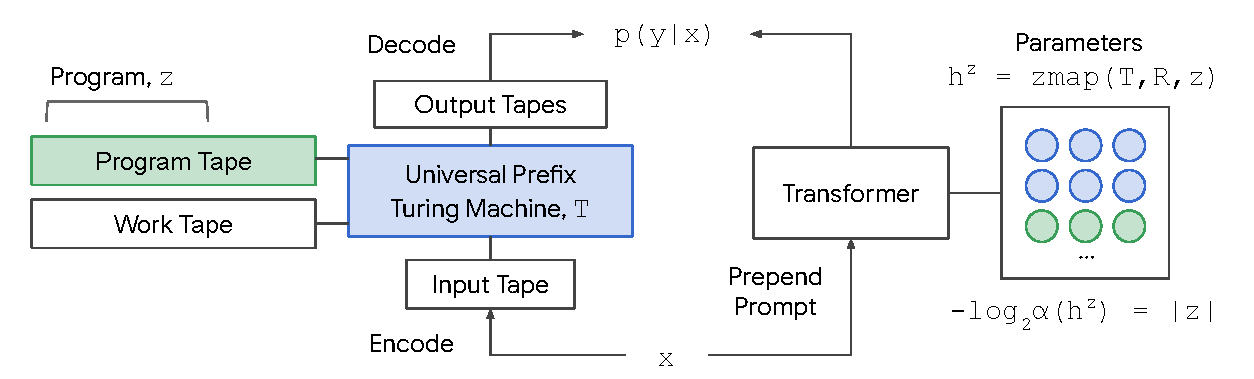
\includegraphics[width=0.75\columnwidth,keepaspectratio]{figures/transformer_turing_emulator_pdf.pdf}
    \caption{\textbf{Constructing asymptotically optimal codes for Transformers.} We construct a function $\zmap$ that establishes that a Transformer (right) can effectively simulate a prefix Turing machine $T$ with any prefix $z$ encoded on a program tape (left), and therefore can represent any computable model function (as defined in section~\ref{sec:problem-setting}) within some arbitrary time and space resource bound $R$. With this mapping between model functions and Transformer parameters established, we can select a prior that assigns probability to sets of parameters based on the algorithmic complexity of the function they compute, thus forming an asymptotically optimal code (Section~\ref{sec:two-part-codes-for-transformers}).}
    \label{fig:transformer_turing_emulator}
\end{figure}


\subsection{Two-part codes for Transformers}
\label{sec:two-part-codes-for-transformers}

The Transformer architecture~\citep{vaswani2017attention} defines a family of models with various hyperparameters determining the time (e.g., number of layers) and space (e.g., context window size) resources of the model. We focus our theoretical analysis on Transformer \emph{encoders}
applied to sequence classification, a commonly studied setting
\cite[e.g.,][]{devlin2019bert}.

\begin{thm}\label{thm:transformer-two-part-code}
There exists an \emph{asymptotically optimal} family of two-part codes for Transformer encoders.
\end{thm}

Figure~\ref{fig:transformer_turing_emulator} captures the main idea.
Given a universal prefix Turing machine $T$ and resource bound $R$, let $\gZ_{T,R}$ denote the set of programs such that $T$ halts within $R_t$ steps and requires only up to $R_s$ registers on any tape, for any input $x \in \gX$ encoded on the input tape. Let $f^z_T: \gX \rightarrow \gL$ be the \emph{model function} computed by $T$ with prefix $z$ on the program tape. For a given $R$, we construct a two-part code $M_R$ where the hypothesis space $\gH_{M_R}$ and mapping function $m_{M_R}$ are defined by a Transformer encoder, with $\gO(R_t)$ layers and a context window size of $\gO(R_s)$. 
We use ALTA~\citep{shaw2024alta}, a compiler from symbolic programs to Transformer weights, to construct a function $\zmap$ such that $\forall z \in \gZ_{T,R},~m_{M_R}(h^z) = f^z_T$ where $h^z = \zmap(T,R,z)$. While future work could consider alternative ways of constructing such a mapping (see \ref{sec:alternative-families}), our particular construction relies on prepending a sequence of $R_s$ ``prompt tokens'' to the model input, with learnable embeddings. These prompt tokens represent the program $z$, while the attention and MLP weights are configured to act as an interpreter, emulating the Turing machine $T$. We can then trivially construct a prior $\alpha_{M_R}(h)$ that such that $\forall z \in \gZ_{T,R},~-\log_2 \alpha_{M_R}(h^z) = |z|$, with $\alpha_{M_R}(h) = 0$ for hypotheses outside the range of $\zmap$. This construction can be shown to satisfy the conditions of an asymptotically optimal family of codes with respect to $T$. Further, any prior satisfying the more relaxed condition $\forall z \in \gZ_{T,R},~-\log_2 \alpha_{M_R}(h^z) < |z| + c_T$ where $c_T$ is a constant not depending on $R$ or $z$ is sufficient. (See \ref{sec:app-proof-transformer-two-part-code} for the formal proof.) 

\subsection{Limitations \& Practical considerations}
\label{sec:practical-considerations}

While asymptotically optimal codes offers appealing compression bounds, in this section we discuss why these bounds are insufficient to guarantee real-world performance and relevant practical considerations.

First, the theoretical guarantees  hold in the limit as model resources increase, and hold up to an additive constant that only becomes negligible as dataset complexity increases. While the community has been training increasingly large models on increasingly large datasets, any real-world models and datasets are, of course, finite. For a finite-resourced Transformer, satisfying the conditions of an asymptotically optimal code only formally constrains the description length of a subset of the computable functions that could be represented. Strictly emulating a Turing machine can be inefficient, failing to leverage a Transformer's capacity for parallel and numerical computation. Therefore, intuitively, we should consider sufficiently \emph{general and flexible priors} that are not overly specialized to a specific Turing machine. For a sufficiently flexible prior, our method used to prove asymptotic optimally -- showing that a Transformer can emulate a universal prefix Turing machine -- serves primarily to establish a worst-case upper bound on the minimum achievable codelength. 

Second, the formal guarantees apply to the \emph{minimum} of the codelength objective. Practically, we need to consider objectives that are computationally tractable and can be efficiently optimized.

% The two-part code for Transformers derived in \ref{sec:two-part-codes-for-transformers} is potentially problematic in practice. The prior is overly rigid, assigning zero probability to parameters that don't correspond to emulating a specific Turing machine. The prior also involves complex dependencies between parameters and is non-differentiable with respect to the model parameters, making optimization challenging. However, flexibility in constructing $\zmap$ and the prior enable significant degrees in freedom in constructing asymptotically optimal codes.

% To address these limitations, let us first provide some perspective. The theoretical guarantees of an asymptotically optimal code hold in the limit as dataset complexity and model resource bounds increase, assuming the codelength objective can be perfectly optimized. While the community has been training increasingly large models on increasingly large datasets, any real-world models and datasets are, of course, finite. Strictly emulating a Turing machine can be inefficient, failing to leverage a Transformer's capacity for parallel and numerical computation, and overly restricting the parameter values considered during training can hinder effective optimization. Therefore, in practice, we should consider more flexible codes that enable the optimization process to consider parameter values that make more efficient use of a Transformer's finite computational resources. For a sufficiently flexible code, our method used to prove asymptotic optimally -- showing that a Transformer can emulate a universal prefix Turing machine -- serves primarily to establish a worst-case upper bound on the minimum achievable codelength; it is likely that for any given dataset and finite model, there exists a set of parameters offering a shorter total codelength than the upper bound associated with a literal Turing machine emulation.

Therefore, we should aim to identify codes that are asymptotically optimal (or approximately optimal) but also satisfy these additional informal but intuitive criteria, which can ultimately be assessed empirically.
%\begin{enumerate}[noitemsep, nolistsep]
%    \item Are based on a sufficiently general and flexible prior.
%    \item Can be optimized with standard gradient-based methods.
% \end{enumerate}
As one potential path toward meeting this goal, we consider \emph{variational codes}, which we study theoretically in Section \ref{sec:variational-codes} and empirically in \ref{sec:variational-code-experiments}. We also analyze the asymptotic bounds for various alternative two-part codes in \ref{sec:asymptotic-bounds}. %

\vspace{-0.12cm}
\section{Variational Codes}
\label{sec:variational-codes}
\vspace{-0.1cm}


\begin{figure}[t!]
    \centering
    \scalebox{0.9}{
    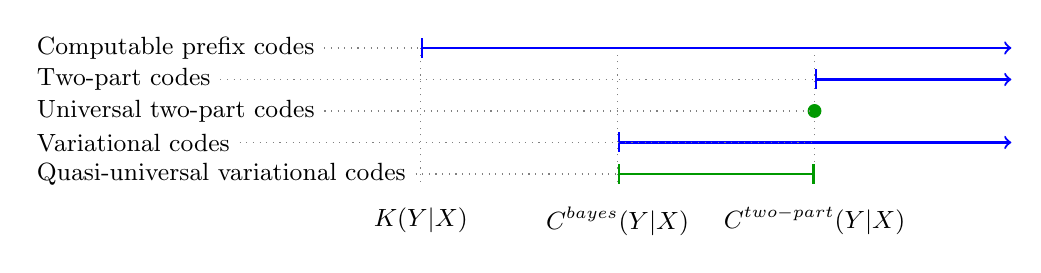
\begin{tikzpicture}[
    axis/.style={thick, ->, >=stealth},
    code_label/.style={anchor=west, font=\small},
    formula_label/.style={below=0.2cm, text width=3.5cm, text centered, font=\small},
    blue_code/.style={blue, thick},
    green_code/.style={green!60!black, thick},
    v_helper_line/.style={thin, dotted, gray},
    h_helper_line/.style={thin, dotted, gray}
]

    \def\xKYX{0}       %
    \def\xUBC{2.5}     %
    \def\xUTPC{5.0}    %
    \def\xInfinity{7.5} %
    \def\xLabelCol{-5} %
    \def\lenVar{1.5}   %

    \def\yPrefix{1.7}      %
    \def\yTwoPart{1.3}     %
    \def\yUTPC{0.9}        %
    \def\yVar{0.5}         %
    \def\yQuasi{0.1}       %


    \coordinate (kyx) at (\xKYX,0);
    \coordinate (ubc) at (\xUBC,0);
    \coordinate (utpc) at (\xUTPC,0);
    \coordinate (infinity) at (\xInfinity,0);

    \draw[v_helper_line] (ubc) -- (ubc |- 0, \yPrefix);
    \draw[v_helper_line] (kyx) -- (kyx |- 0, \yPrefix);
    \draw[v_helper_line] (utpc) -- (utpc |- 0, \yPrefix);
    
    \node[formula_label] at (kyx) {$K(Y|X)$};
    \node[formula_label] at (ubc) 
    {$C^{\text{bayes}}(Y|X)$};
    \node[formula_label] at (utpc)
        {$C^{\text{two-part}}(Y|X)$};

    
    \node[code_label] (prefix_label) at (\xLabelCol, \yPrefix) {Computable prefix codes};
    \draw[blue_code, |->] (kyx |- 0, \yPrefix) -- (infinity |- 0, \yPrefix);
    \draw[h_helper_line] (prefix_label.east) -- (kyx |- 0, \yPrefix);

    \node[code_label] (twopart_label) at (\xLabelCol, \yTwoPart) {Two-part codes};
    \draw[blue_code, |->] (utpc |- 0, \yTwoPart) -- (infinity |- 0, \yTwoPart);
    \draw[h_helper_line] (twopart_label.east) -- (utpc |- 0, \yTwoPart);

    \node[code_label] (utpc_label) at (\xLabelCol, \yUTPC) {Universal two-part codes};
    \fill[green!60!black] (utpc |- 0, \yUTPC) circle (2.5pt);
    \draw[h_helper_line] (utpc_label.east) -- (utpc |- 0, \yUTPC);

    \node[code_label] (var_label) at (\xLabelCol, \yVar) {Variational codes};
    \draw[blue_code, |->] (ubc |- 0, \yVar) -- (infinity |- 0, \yVar);
    \draw[h_helper_line] (var_label.east) -- (utpc |- 0, \yVar);

    \node[code_label] (quasi_label) at (\xLabelCol, \yQuasi) {Quasi-universal variational codes};
    \draw[green_code, |-|] (ubc |- 0, \yQuasi) -- (utpc |- 0, \yQuasi);
    \draw[h_helper_line] (quasi_label.east) -- (ubc |- 0, \yQuasi);
    
        
\end{tikzpicture}

    } %
    \caption{\textbf{Upper and lower bounds on minimum codelengths.} The figure shows the minimum number of bits required to transmit labels $Y$ given inputs $X$, for different classes of codes. The bounds hold for any dataset ($X,Y$) up to an additive constant that does not depend on the dataset.}
    \label{fig:codelength_comparisons}
\end{figure}


An alternative approach for Alice to transmit the data labels to Bob is to use a \emph{variational code}, which considers a \emph{distribution} over hypotheses, rather than selecting a single best hypothesis. We start with some definitions and formal results, and then work towards a practical implementation.

\begin{defn}[variational code]
A \emph{variational code} $M$ consists of a hypothesis space $\gH_M$, a mapping $m_M : \gH_M \rightarrow \gF$ from hypotheses to model functions, and prior $\alpha_M(h)$ over $\gH_M$, as specified in definition~\ref{def:two-part-code}. Additionally, a variational code specifies a posterior hypothesis space, $\Phi_M$, and distribution over hypotheses, $\beta_M(h;\phi)$, parameterized by $\phi \in \Phi_M$.
\end{defn}

The conditional distribution over $Y$ given $X$ is therefore specified by the posterior parameters $\phi \in \Phi_M$, and defined by marginalizing over hypotheses:
\begin{equation}
p_M(Y \mid X; \phi) = \mathbb{E}_{h \sim  \beta_M(\cdot;\phi)} ~p(Y \mid X;m_M(h)).
\end{equation}
The codelength for a variational code $M$ is then defined as:
\begin{align}
L_M^{\text{var}}(Y \mid X,\phi) &= \mathbb{E}_{h \sim \beta_M(\cdot;\phi)} \left[
-\log_2~\alpha_M(h) + \log_2~\beta_M(h;\phi) - \log_2~p(Y \mid X; m_M(h))
\right] \label{eq:variational-code} \\
 &= \text{KL}\left[ \beta_M(\cdot;\phi) \parallel \alpha_M(\cdot) \right] - \log_2~ p_M(Y \mid X; \phi), \label{eq:variational-code-kl} 
\end{align}
which can be interpreted as the cost of transmitting the labels given the ``bits back'' argument of \citet{hinton1993keeping}.
The intuition is that parameters with higher uncertainty can be transmitted with lower cost. Equation~\ref{eq:variational-code-kl} mirrors \eqref{eq:two-part-code}, with the KL term capturing the model cost.
We denote the minimum of a variational code $M$ as:
\begin{equation}
L_M^{\bigast,\text{var}}(Y \mid X) = \min_{\phi \in \Phi_M}~ L_M^{\text{var}}(Y \mid X,\phi).
\end{equation}
A variational code can be seen as approximating an idealized but intractable Bayesian code (\ref{sec:bayesian-lower-bound}). As with two-part codes, variational codes require choosing a seemingly arbitrary prior.
We address this by defining \emph{quasi-universal variational codes}, which are analogous to universal two-part codes.

\begin{defn}[quasi-universal variational code]
A variational code $M$ is a \emph{quasi-universal variational code} if and only if:
\begin{equation}
L^{\bigast,\text{var}}_{M}(Y \mid X) \leqc C^{\text{two-part}}(Y \mid X).
\end{equation}
\end{defn}


We use the term \emph{quasi-universal} because such codes are not necessarily strictly universal among the set of variational codes. However, their minima are tightly bound per the following theorem.

\begin{prop}\label{thm:codelength-relations}
For any quasi-universal variational code $M$,
\begin{equation}
    K(Y \mid X) \leqc C^{\text{bayes}}(Y \mid X) \leqc L^{\bigast,\text{var}}_{M}(Y \mid X) \leqc C^{\text{two-part}}(Y \mid X),
\end{equation}
where $C^{\text{bayes}}(Y \mid X) := -\log_2 \sum_{f \in \gF} 2^{-K(f)} p(Y \mid X;f)$.
\end{prop}

The result is visualized in Figure~\ref{fig:codelength_comparisons}. The proof involves deriving $C^{\text{bayes}}(Y \mid X)$ as the minimum of a universal Bayesian code (\ref{sec:proof-of-thm-codelength-relations}). Under reasonable conditions, the differences between each of these quantities are expected to be small. See \ref{sec:relations-between-codes} for formal analysis and discussion.
The definition of asymptotically optimal families of two-part codes directly extends to variational codes (\ref{sec:asymptotically-optimal-var-codes}). %
Additionally, variational codes can be seen as a generalization of two-part codes (\ref{sec:var-two-part-equivalence}), and therefore our previous result constructing asymptotically optimal two-part codes for Transformers directly extends to prove the following proposition (\ref{sec:proof-of-exists-asymptotically-optimal-code}).

\begin{prop}\label{thm:exists-asymptotically-optimal-code}
There exists an asymptotically optimal family of variational codes for Transformer encoders. 
\end{prop}

Finally, we note that we can also generalize variational codes by using an \emph{adaptive prior}~\citep{hinton1993keeping}, where the prior is itself parameterized. We term such codes \emph{adaptive variational codes}, defined formally in~\ref{sec:adaptive-prior}. Adaptive priors help generalize our previously constructed codes to form a more flexible implementation, discussed next.

\subsection{Differentiable Codes via Gaussian Mixture Models}
\label{sec:transformer-practical-code}

Per the discussion in~\ref{sec:practical-considerations}, we aim to identify families of asymptotically optimal codes for Transformers that are based on flexible and general priors -- not explicitly constructed around a specific Turing machine emulation -- and are amenable to standard gradient-based optimization.
As one path towards this goal, we construct a family of adaptive variational codes where the adaptive prior and posterior distributions are both parameterized by sets of independent Gaussian mixture models (GMMs; see~\ref{sec:gaussian-parameterization}). Intuitively, a GMM prior shared across a group of weights drives compression by encouraging a low-entropy clustering of weight values around the component means, akin to soft quantization~\citep{ullrich2017soft,achterhold2018variational,han2016deep}. Such a GMM-based construction is appealing for its generality, and because we can estimate the variational codelength objective using Monte-Carlo sampling and apply standard optimizers via the reparameterization trick~\citep{kingma2014auto,jang2017categorical,maddison2017concrete}. The proof of Theorem~\ref{thm:gmm-code-is-optimal} below demonstrates that this construction is also asymptotically optimal, thus establishing a worst-case asymptotic upper bound on the minimal codelength (i.e. compression) achievable with such codes. The proof also serves to illustrate a potential path towards identifying other instances of practical and asymptotically optimal codes.

\begin{thm}\label{thm:gmm-code-is-optimal} There exists an asymptotically optimal family of adaptive variational codes for Transformer encoders where the adaptive prior and posterior distributions are both specified by products of independent GMMs.
\end{thm}

The key challenge in satisfying this theorem, in contrast to our earlier existence proofs, lies in the stronger constraints imposed on the prior distribution, particularly the independence assumptions. We show that two relatively general conditions are sufficient to establish asymptotic optimality. First, we use layerwise weight sharing, as in a Universal Transformer~\citep{dehghani2019universal}, ensuring that the number of Transformer weights doesn’t scale with the time bound $R_t$. Second, we share a GMM prior over groups of Transformer weights, ensuring that the number of prior parameters doesn't scale with the space bound $R_s$.

The formal proof is in~\ref{sec:transformer-var-code-details}. Our proof sketch here builds on the function $\zmap$ and the related notation introduced in Section~\ref{sec:two-part-codes-for-transformers}. Given a universal prefix Turing machine $T$, for every resource bound $R \in \gR$ and program $z \in \gZ_{T,R}$, we construct GMM posterior parameters $\phi^{R,z}$ and GMM prior parameters $\psi^{R}$ such that the KL divergence is equal to $|z|$ plus an additive constant and the model function is deterministic and equivalent to $f_T^z$. Specifically, we construct $\phi^{R,z}$ to approximate a delta function at each weight in $\zmap(T,R,z)$, except for weights representing the program tape past the $|z|$th register; these weights do not affect the model function being computed, and we therefore set their posterior to be equal to their respective prior, such that they can be transmitted ``for free''.
Importantly, by construction, the output of $\zmap$ consists of a constant number of weights (depending on $T$ but not $R$) outside of the $R_s$ prompt embeddings (which represent the program tape contents). By sharing a GMM prior across each feature column of the prompt embeddings table, the total KL for these embeddings is shown to be $|z|$ bits.
The fixed number of remaining weights can be transmitted in a constant number of bits for any GMM prior assigning non-zero probability to the associated weights in $\zmap(T,R,z)$. This establishes the necessary upper bound on the minimum codelength, although there may be prior and posterior parameters offering even greater compression.


